\documentclass{article}
\usepackage[utf8]{inputenc}
\usepackage{graphicx}
\usepackage[dutch]{babel}
\usepackage{xcolor}
\usepackage[framemethod=default]{mdframed}
\usepackage{tocloft}
\usepackage{adjustbox}
\usepackage{pbox}
\usepackage{enumitem}
\usepackage{comment}


\usepackage{chngcntr}
\counterwithout{subsection}{section}
% Question command
\newtheorem{qtext}{Question}
\let\olddefinition\qtext
\renewcommand{\qtext}{\olddefinition\normalfont}

\makeatletter
\renewcommand*{\@seccntformat}[1]{\csname the#1\endcsname\hspace{0.2 cm}}
\makeatother

\renewcommand{\thesubsection}{Chapter \arabic{subsection} -}
\renewcommand{\thesection}{Part \arabic{section} -}

% Set text counters
\setcounter{qtext}{0}
\setcounter{section}{0}

\NewDocumentEnvironment{quest}{o}
 {\IfNoValueTF{#1}
   {\question\addcontentsline{toc}{subsection}{\protect\numberline{\thesubsection}Vraag}}
   {\question\addcontentsline{toc}{subsection}{\protect\numberline{\thesubsection}Vraag: #1}}%
   \ignorespaces}
 {\stepcounter{subsubsection}\endquestion}


% Define layout QuestionBox
\newmdenv[skipabove=7pt,
skipbelow=7pt,
rightline=false,
leftline=false,
topline=true,
bottomline=false,
linecolor=gray,
backgroundcolor=black!8,
innerleftmargin=5pt,
innerrightmargin=5pt,
innertopmargin=5pt,
leftmargin=0cm,
rightmargin=0cm,
linewidth=2pt,
innerbottommargin=5pt]{qbox}
\newenvironment{question}{\begin{qbox}\begin{qtext}}{\end{qtext}\end{qbox}}

\addtolength{\cftsecnumwidth}{20pt}
\addtolength{\cftsubsecnumwidth}{25pt}
\renewcommand\cftsecfont{\bfseries}
%----------------------------------------------------------------------------------------
%	TITLE PAGE
%----------------------------------------------------------------------------------------

\newcommand*{\titleGM}{\begingroup % Create the command for including the title page in the document

\hbox{ % Horizontal box
\hspace*{0.2\textwidth} % Whitespace to the left of the title page
\rule{1pt}{\textheight} % Vertical line
\hspace*{0.05\textwidth} % Whitespace between the vertical line and title page text
\parbox[b]{0.75\textwidth}{ % Paragraph box which restricts text to less than the width of the page

{\noindent\Huge\bfseries Requirements \\[0.2\baselineskip] Engineering \large(D0H56A)}\\[2\baselineskip] % Title
{\large \textit{Oplossingen (theoretische) examenvragen}}\\[4\baselineskip] % Tagline or further description
{\Large \textsc{Robin Haveneers}}\\[0.5\baselineskip]
{\small Ge\"updatet en vertaalde versie van het originele document door\\ \textbf{Maarten Rimaux} \& \textbf{Xander Deseyn}\\[4\baselineskip]
{\footnotesize Vertaald naar het Nederlands aangezien het examen\\ ook in het Nederlands is.}}


\vspace{0.4\textheight} % Whitespace between the title block and the publisher
{\noindent 
\includegraphics[scale=0.15]{kul.jpg}}\\[\baselineskip] % Publisher and logo
}}
\endgroup}

%----------------------------------------------------------------------------------------
%	BLANK DOCUMENT
%----------------------------------------------------------------------------------------

\begin{document}

\begin{titlepage}
\pagenumbering{gobble}
\pagestyle{empty}
\titleGM % This command includes the title page
\end{titlepage}

\newpage

\section{Fundamentals and Framework}
\pagenumbering{arabic}
\pagestyle{plain}
\subsection{Motivation}
\vspace{5mm}
\begin{quest}
What zijn de grootste uitdagingen bij het ontwikkele van software-intensieve systemen?
\end{quest}

\begin{itemize}
    \item Innovaties op vlak van software
    \item Toenemende complexiteit (door een groter wordende integratie)
    \item Druk om kosten laag te houden
    \item Verkorten van ontwikkeltijden
    \item Vereiste m.b.t hogere kwaliteit
\end{itemize}

\begin{quest}{}
Wat is het belang van Requirements Engineering?
\end{quest}Het heeft een grote impact op het slagen van een project en de kosten die ermee gepaard gaan.
    \begin{itemize}
    \item Veel projecte falen or slagen pas na de deadline en/of met meer uitgaven dan voorzien en/of met een meer gelimiteerde functionaliteit
    \item Fouten op vlak van requirements zijn de oorzaak voor ongeveer 50\% van het falen van projecten (omwille van onjuistheid, onvolledigheid of inaccuraatheid)
    \item De kosten geassocieerd met requirements engineering propageren zich door de ontwikkelingscyclus.
    \end{itemize}

\begin{quest}{}Welke interrealties bestaan er met andere organisationele processen?
\end{quest}
\begin{itemize}
\item \textit{Requirements engineering en product management}\\
$\Rightarrow$ Product management voorziet het requirements engineering proces van een `product roadmap', productstrategie and `key requirements'. Het requirements engineering proces op zijn beurt levert nieuwe en herwerkte requirements.
\item \textit{Requirements engineering en marketing}\\
$\Rightarrow$ Het marketing proces voorziet de noden van de markt, trends een prijsinterval. Het requirements engineering proces speelt nieuwe features door.
\item \textit{Requirements engineering en customer relationship management} \\
$\Rightarrow$ Het customer relationship management proces bericht over de wensen van klanten en gerapporteerde problemen. Het requirements engineering proces overhandigt gerealiseerde wijzigingen en verbeteringen.
\end{itemize}
\begin{quest}{}
Welke interrelaties bestaan er met andere ontwikkelingsactiviteiten?
\end{quest}
\begin{itemize}
\item \textit{Requirements engineering en project management} \\
$\Rightarrow$ Het requirements engineering proces overhandigt monitoring data en opgestelde doelen aan het project management proces. Dit proces zorgt op zijn beurt voor een projectplan en goedgekeurde doelen.
\item \textit{Requirements engineering en design} \\
$\Rightarrow$ Het requirements engineering proces zorgt voor requirements en constraints. Het design proces overhandigt met oplossingen en nieuwe technologie\"en.
\item \textit{Requirements engineering en system maintenance} \\
$\Rightarrow$ Het requirements engineering proces rapporteert de status van `change requests' aan het system maintenance proces en zij bezorgen op hun berut de effectieve `change requests'.
\item \textit{Requirements engineering en quality assurance} \\
$\Rightarrow$ Het requirements engineering proces communiceert de requirements artefacts aan het quality assurance process zij bezorgen verbetering en kunnen eventuele verduidelijkingen opvragen.
\end{itemize}

\subsection{Requirements}

\begin{quest}{}Welke verschillende types van requirements kunnen we onderscheiden? Leg kort uit en illustreer met een voorbeeld.
\end{quest}

\begin{itemize}
    \item Functionele requirements: \\
    Services die het systeem moet voozien, de mogelijkheid om te reageren op bepaalde inputs, gedrag van het system en zaken die het systeem niet zou mogen doen.\\
    $\Rightarrow$ Hoofdzakelijk `solution-oriented' requirements gedocumenteerd op basis van het data-, functioneel- en `behavioural'-perspectief.\\
    \textit{Voorbeeld: Als de gebruiker een correcte toegangscode invoert, zal het systeem de deur openen en toegang verlenen.}
    \item Kwaliteits requirements: \\
    Definieert kwaliteitseigenschappen van het systeem, component of service (vb. service-level agreements).\\
    $\Rightarrow$ Er bestaat een verschil tussen `quality requirements' naar gebruikers toe (beschikbaarheid, flexibiliteit ...) en naar ontwikkelaars toe (onderhoudbaarheid, herbruikbaarheid...).\\
      \textit{Voorbeeld: Het systeem moet een gebruiksvriendelijke interface voorzien.}\\
      \textbf{Opmerking} - Deze maken een deel uit van zogenaamde \textit{`non-functional requirements' (NFR)} echter bestaat deze term niet echt aangezien ze bestaan uit kwaliteits requirements en een hoop te weinig gespecifieerde functionele requirements.
    \item Voorwaarden: \\ 
    Organisationele of technologische requirement de welke een restrictie vormt bij het ontwikkelen van het systeem.\\
    $\Rightarrow$ Er zijn verschilende types onder te brengen op basis van hun oorsprong of geen waar ze effect op hebben.\\
    \textit{Voorbeeld: Het systeem zal ten laatste beschikbaar zijn op 1 Mei 2017.}
\end{itemize}

\begin{quest}{}Leg uit wat bedoeld wordt met``Problem versus Solution" en hoe dit een rol speelt in requirements engineering.
\end{quest}

\begin{itemize}
    \item ``Wat (problem) vs. ``Hoe?” (solution) \\
    $\rightarrow$ "Wat?" =  Omschrijving van het probleem\\
     $\rightarrow$ "Hoe?" = Omschrijving van de oplossing. \\
     Deze zijn afhankelijk van de verschillende visies van de stakeholders.
    \item Het effect van deze aanpak is dat de `solution space' afneemt tijdens het ontwikkelingsproces.
    \item Interactie tusen requirements engineering en de `design space' (``twin-peaks model")\\
    $\Rightarrow$ Ontwerpbeslissingen leiden tot modificatie en verfijning van de initiële, ``grofkorrelige'' requirements (= een groot deel van de requirements zijn opgesteld met een preliminaire oplossing in gedachten).
\end{itemize}

\subsection{Continuous requirements engineering}

\begin{quest}{}
Bespreek het conept `Traditional System Analysis'. Wat is het? Wat is het mis mee.
\end{quest}
Methodes gebruikt voor een traditionele systeemanalyse:
\begin{itemize}
	\item Analyse van de huidege toestand (documenten van reeds behaalde requirements, contextinformatie en mogelijkheden tot verbeteringen)
	\item Vastleggen van de gewenste toestand (in acht nemen van geefinieerde verbteringen, vastleggen van de requirements)
\end{itemize}
Probleem: een `desired-state model' mag niet vooringenomen worden door technologische of implementationele overwegingen (van het bestaande, huidge systeem). 

\begin{quest}{}Bespreek het conept `Essential System Analysis'. Wat is het? Wat is er `goed' aan?.
\end{quest}
\begin{itemize}
    \item Het is een oplossing voor het probleem met de structurele analyse: er wordt namelijk een onderscheid gemaakt tussen essentie en incarnatie van het systeem.
    \item Essentie (essentieel model): een systeemontwerp dat zou bestaan moest de technologie nodig om het te implementeren perfect zijn (en er dus geen technische limitaties bestonden): perfecte processoren, data-containers...
    \item Incarnatie (fysiek model): opsomming van `real-life' objecten nodig om het systeem te implementeren (rekening houdend met de beperkingen van de technologie).
\end{itemize}
Essenti\"ele modellen zijn stabieler en minder afhankelijk van technologische veranderingen, kleiner en bijgevolg gemakkelijker om te gebruiken en aan te passen. Ze hebben geen restricties op vlak van design en zijn vaak hetzelfde voor bestaande en nieuwe systemen.

\begin{quest}{}Bespreek `phase-oriented' versus `continuous requirements engineering': wat wordt bedoeld met deze termen, wat zou de gepreferreerde aanpak zijn en waarom?
\end{quest}

\begin{itemize}
	\item Phase-oriented: \\
Requirements engineering wordt beschouwd als een enkelvoudige, vroege fase in het ontwikkelingsproces
\begin{itemize}
 \item Requirements worden niet ge\"updatet tijdens het ontwikkelingsproces.
 \item Elk nieuw proces vereist een tijdsintensieve `current-state' analyse.
 \item Geen hergebruik van requirements
 \item Enge, nauwe focus op \'e\'en product met als gevolg dat relevante informatie over het hoofd wordt gezien.
 \end{itemize}
	\item Continuous \\
	Requirements zijn een `cross-lifecycle', `cross-project', `cross-product' activiteit. De voordelen van het delen van een gemenschappelijk subject domein tussen korte productlevenscycli en een project, zijn de volgende.
	\begin{itemize}
	\item Duidelijke requirements basis
	\item Requirements blijven up-to-date
	\item Kortere ontwikkeltijden (vermijden van de `current-state' analyse.
	\item Hergebruik van requirements artefacten
	\item Duidelijke verantwoordelijkheden, ongeacht het projectpersoneel.
	\end{itemize}
\end{itemize}

\subsection{The requirements engineering framework}

\begin{quest}{}Wat zijn de vier context facetten van  requirements engineering ? Omschrijf ze kort en vermeld ook de onderlinge relaties.
\end{quest}
\textbf{Mnemonisch: SUITeD}
\begin{enumerate}
	\item Subject (onderwerp) facet: \\
	= `domein'
	Objecten en gebeurtenissen relevant voor het systeem. Zaken die het systeem moet opslaan of waarover het informatie moet verwerken.
	\item Usage (gebruik) facet: \\
	= `door wie gebruikt, in welke volgorde ...'\\
	Aspecten gerelateerd aan het gebruik door mensen of andere systemen (vb. gebruiksdoelen (`usage goals'), workflows, interfaces ...)
	\item IT system facet: \\
	= `technolgie om het systeem te bouwen'\\
	Objecten en elementen van de infrastructurele en architecturale IT-omgeving van het systeem (vb. bestaande hardware en software die dienen te worden gebruikt omwille van strategische of architecturale IT beslissingen).
	\item Development (ontwikkeling) facet: \\
	= `alles dat de ontwikkeling aanstuurt'\\
	Aspecten met betrekking tot de ontwikkeling van het systeem (vb. proces richtlijnen, ontwikkelingstools, standaarden op gebied van kwaliteitsgarantie).
\end{enumerate}

\begin{quest}{}Wat zijn de drie dimensies van requirements engineering? Omschrijf ze kort en formuleer die hieropvolgende essenti\"ele doelen van requirements engineering.
\end{quest}
= drie kernactiviteiten \& overeenkomstige doelen van requirements engineering
\begin{enumerate}
    \item Inhoudelijke (content) dimensie - elicitatie/ontlokking: \\
    \textit{vague $\rightarrow$ complete}\\
    Al de relevante requirements zijn expliciet gekend en verstaan op het gewenste niveau van detail. De requirements worden ontrokken via stakeholders en andere requirements bronnen.
    \item Akkoordelijke (agreement) dimensie - onderhandeling: \\
    \textit{individual views $\rightarrow$ consolidated views}\\
    Men moet een voldoende goed akkoord bereiken tussen verscchillende stakeholders. Vinden en oplossen van conflicten tussen stakeholders.
    \item Documentatie (documentation) dimensie - documentatie: \\
    \textit{informal $\rightarrow$ compliant with rules}\\
    Alle requirements moeten gedocumenteerd zijn conform de regels.
    Voor documentatie zijn er verscheidene regels.
    \begin{itemize}
    \item Algemene documentatieregels: alle soorten informatie (bv. meta-data van documenten)
    \item Documentatieregels: documentatieregels voor elke fase van het proces (vb. templates)
    \item Specificatieregels: documenteren van requirements die in de requirements specificatie leven (vb. regels van de modelleertaal)
    \end{itemize}
\end{enumerate}

\begin{quest}{}What are the two cross sectional activities of Requirements Engineering ? Briefly describe each of them.
\end{quest}

\begin{enumerate}
	\item Validation/validatie: nakijken/verbeteren van ``core activities'' (= `compliance checking'), ``requirement artefacts'' (rekening houdend met de drie dimensies) and ``system context''.
	\item Management/beheer: beheren/onderhouden van ``activities'' (planning en controler), ``requirement artefacts'' (doorheen cyclus) and ``system context'' (monitoren van veranderingen).
\end{enumerate}

\begin{quest}{}Wat zijn de drie types van `requirement' artefacten? Beschrijf ze elk bondig.
\end{quest}

\begin{enumerate}
	\item Goals/doelen: de intenties van de stakeholders, abstract van het gebruike (=`solution free'). Ze hebben vaak een voorschrijvende aard en ondersteunen conflictresolutie. Deze leiden tot een betere verstaanbaarheid van het systeem en toenemend aanvaarding.
	\item Scenarios: Een concreet voorbeeld van het slagen of falen van een goal/set of goals. Hoofdzakelijk uiteengezet in een sequentie of interactie van stappen.
	\item Solution-oriented requirements/oplossingsgerichte requirements: specifi\"eren de data-, functionele en gedragsperspectieven van het software-intensieve systeem. Ze omvatten de solution-oriented requirements zelf en constraints. Ze impliceren vaak een conceptuele oplossing voor het systeem.
\end{enumerate}


\section{System Context}

\subsection{System and Context boundaries}

\begin{quest}{}Verklaar de volgende concepten en hun rol in requirements engineering: `system' en `context' grenzen/`boundaries'.
\end{quest}

\begin{itemize}
    \item System boundary/systeemgrens:\\
     Scheiding tussen variabele en stabiele artefacten. Initieel is deze maar vaag omschreven (de zogeheten `grey zone'). Latere aanpassingen tijdens de ontwikkeling zullen deze gres nog doen wijzigen.
    \item Context boundary/contextgrens:\\
     Verdeelt de contextuele aspecten in twee groepen.
     \begin{enumerate}
     \item Relevante aspecten van de systeemcontext
     \item Irrelevate aspecten van het omgevingsaspect (buiten beschouwing tijdens de ontwikkeling)
     \end{enumerate}
     Ook deze grens (met name kennis over relevantie van bepaalde contextaspecten) wijzigt over het algemeen nog tijdens het requirements engineering proces. 
\end{itemize}

\subsection{Structuring the system context}

\begin{quest}{}Verklaar de volgende concepten en hun rol in requirements engineering: `subject'/onderwerp, `usage'/gebruik facet, IT systeem facet, `development'/ontwikkelingsfacet.
\end{quest}

\begin{itemize}
    \item `Subject'/onderwerp facet\\
    Objecten en events die moeten worden gerepresenteerd in het systeem.
    \item `Usage'/gebruiksface\\
    Alle aspecten aangaande het gebruik van het systeem door mensen en andere systemen.
    \item IT system facet\\
    De aspecten aangaande de technische of operationele omgeving waarin het systeem is gedefinieerd, onder meer software en hardware componenten maar ook IT strategie\"en, architecturen en beleid.
\end{itemize}


\begin{quest}{}(Mogelijke alternatieve versie van de vorige) Verklaar de volgende concepten en hun rol in requirements engineering: requirement `sources'/bronnen, context `objects'/objecten, `properties'/eigenschappen en `relationships'/relaties tussen context objecten. 
\end{quest}

\begin{itemize}
    \item Requirement `sources'/bronnen\\
    De oorsprong van de requirements vastgelegd voor het systeem. Onder meer: stakeholders, bestaande documentatie en andere bestaande systemen.
    \item Context `objects'/objecten\\
    Mensen of objecten in een bepaalde context die moeten betrokken of overwogen worden tijdens requirements engineering. OVer deze objecten/mensen moet data worden bijgehouden in het systeem.
    Onder meer personen, legale entiteiten, materi\"ele objecten en immateri\"ele objecten.
    \item `Properties'/eigenschappen en `relationships'/relaties tussen context objecten\\
    Stellen additionele informatie voor over de context objecten en karakteriseren een context meer in detail.
\end{itemize}

\begin{adjustbox}{center}
\begin{tabular}{p{0.3\linewidth}|p{0.4\linewidth}|p{0.4\linewidth}|p{0.4\linewidth}|}
\centering
\pbox{20cm}{\textbf{\textit{Context aspects $\rightarrow$}} \\ \textbf{\textit{Context facets $\downarrow$}}}& \textbf{Requirements sources} & \textbf{Context objects} & \textbf{Properties \& Relationships}\\ \hline
\vspace{1.2cm}\textbf{Subject} & 
\begin{itemize}[leftmargin=*] 
\item Domain experts, relevant stakeholders 
\item Reference models 
\item Existing systems 
\end{itemize} & 
\begin{itemize}[leftmargin=*] 
\item Persons data is stored about \item Material objects, immaterial objects \item Processes 
\end{itemize} & 
\begin{itemize}[leftmargin=*] 
\item Relevant properties
\item Mapping function defining representation of context objects
\end{itemize}  \\ \hline
\vspace{1.2cm}\textbf{Usage} & 
\begin{itemize}[leftmargin=*] 
\item (In)direct users, experts for UI
\item Standards, laws, regulations
\item Existing systems 
\end{itemize}
& 
\begin{itemize}[leftmargin=*] 
\item User groups
\item Input modality, usage workflows
\item Usage by other systems
\end{itemize}
&  
\begin{itemize}[leftmargin=*] 
\item Relationships between workflows, and between user groups and workflows
\item Relationships to the IT system facet \& subject facet
\end{itemize}
\\ \hline
\vspace{1.2cm}\textbf{IT System} &
\begin{itemize}[leftmargin=*] 
\item Persons dealing with planning, design, operation of IT system
\item IT infrastructure documents
\item Analysis of existing systems
\end{itemize}
&
\begin{itemize}[leftmargin=*] 
\item Hardware \& software components
\item Operation an maintenance
\item IT strategies, policies, architecture
\end{itemize}
&  
\begin{itemize}[leftmargin=*] 
\item Technical data of hardware \& software
\end{itemize}
\\ \hline
\vspace{1.2cm}\textbf{Development} & 
\begin{itemize}[leftmargin=*] 
\item Porcess stakeholders (process engineers, managers \& executors)
\item Guidelines for the development process
\end{itemize}
& 
\begin{itemize}[leftmargin=*] 
\item Role definitions, artefact definitions, activity definitions, tools, resource availability \& restritions
\end{itemize}
&  \\ \hline
\end{tabular}
\end{adjustbox}

\newpage

\section{Requirements artefacts}

\subsection*{A \& B: Goals \& Scenarios}

\begin{quest}{}Bespreek het concepts `goals' als een requirement artefact.\end{quest}
Een goal is een intentie van een belanghebbende/stakeholder met inbegrip van de doelen, eigenschappen en gebruik van het systeem. De motivatie bestaat uit de volgende deelelementen:
\begin{itemize}
    \item Een gemeenschappelijk begrip van het systeem voorzien
    \item Ondersteunen van requirements-ontlokking
    \item Ontdekken en evalueren van alternatieve realisaties
    \item Vinden van irrelevante requirements
    \item Staven van requiremnets
    \item Bewijs van compleetheid voor requirements-specifcaties
    \item Vinden en verhelpen van conclicten
    \item Goals hebben over het algemeen een grotere `stabiliteit'
\end{itemize}
Documentatieregels voor goals
\begin{enumerate}
    \item Beknopt maar niet te nauw
    \item Actief
    \item Documenteer stakeholder's intentie nauwgezet
    \item Ontleed `high-level' goals
    \item Geef de waarde van een goal aan
    \item Geef motivering voor een doel
    \item Vermijd restricties, probeer bestaande restricties te verzwakken
\end{enumerate}
Goal Modelling Languages:
\begin{itemize}
	\item I*, gebaseerd op GRL (Strategic Dependency Model en Strategic Rational Model)
	\item AND/OR graph/tree
\end{itemize}


\begin{quest}{}Bespreek het concept van scenario's als requirements artefact en het gebruik ervan in systeemontwikkeling.
\end{quest}
Scenario's zijn `middle-level abstractions'. De motivering is de volgende:
\begin{itemize}
	\item Goals alleen zijn niet voldoende ondersteunend bij requirements-ontlokking\\
    $\rightarrow$ Het is eenvoudiger om voorbeelden te gebruiken om requirements over te brengen.
    \item Scenarios zijn tussenliggende abstracties tussen abstracte modellen en de realiteit\\
    $\rightarrow$ Een scenario illustreert hoe aan doelen voldaan wordt door middel van een concrete opeenvolging van interacties tussen het systeem en de gebruiker.
\end{itemize}
Documentatieregels:\\
Narratieve scenarios:
\begin{itemize}
    \item `Natural language'
    \item Opeenvolging van interacties als kort verhaaltje (descriptief, verkennend, beschrijvend - hoofd, alternatieve en exceptionele stappen)
    \item Verschillende niveau's van abstratie (minder belangrijk = meer abstract)
\end{itemize}
Structured scenarios:
\begin{itemize}
    \item Better readability/comprehensibility
    \item Enumeration vs tabular documentation
    \item Reference template for scenarios\\
\end{itemize}
Voorgesteld in (UML) sequence diagrams, activity diagrams of use case diagrams.

\begin{quest}{}Geef en verklaar de verschillende soorten scenariotypes.\end{quest}
\begin{itemize}
    \item Current-state (as-is)/indicatief en desired-state (optatief) scenario's
    \item Positive (voldoening aan doel) en negative (falen van een doel) scenarios
    \item Misuse/abuse scenario's
    \item Descriptive, exploratory en explanatory scenario's
    \item Instance (concrete sequentie) en type scenario (abstracte vorm van instance)
    \item Mixed scenario's (combinatie van instance \& type, belangrijke content op instance-niveau)
    \item System-internal, interaction en context scenario's
    \item Main, alternative en exception scenario's
\end{itemize}

Ook hier zijn 11 documentatieregels, maar dit wordt niet expliciet gevraagd.

\begin{quest}{}Wat zijn de voordelen van het gebruik van goals?
\end{quest}
\begin{itemize}
    \item Initialiseren de definitie van scenario's
    \item Zorgen voor de classificatie van scenario's (main, alternative, exception, misuse)
\end{itemize}
Op basis van de volgende aspecten, vinden meer algemeen we de volgende voordelen:
\begin{itemize}
    \item Documentatie: analyseer requirements voor compleetheid en irrelevantie
    \item Ontlokking: basis voor het kiezen van requirements
    \item Onderhandeling: detecteren en oplossen van conflicten tussen stakeholders
    \item Validatie: 'deugdelijkheid' kan worden gecontroleerd op basis van het goal-model
    \item Management: je kan prioriteren op vlak van goals
\end{itemize}
\begin{quest}Wat zijn de voordelen bij het gebruk van sceneario's?\end{quest}
\begin{itemize}
\item Interactiesequenties illustreren het al dan niet voldoen aan goals.
\item Scenario's zorgen voor de initiatie van nieuwe en uitbreiding van bestaande goals (nieuwe sub-goals, nieuwe onafhankelijke goals, verwijderen van goals).
\end{itemize}
Meer algemeen vinden we de volgende voordelen:
\begin{itemize}
    \item Documentatie: richtlijnen voor requirements en structuur
    \item Ontlokking: verfijnen van goals, intentie nader verklaren
    \item Onderhandeling: oplossen van conflicten
    \item Validatie: detecteren van irrelevante doelen en valideren van andere artefacten
    \item Management: prioriteren gebaseerd op scenario's
\end{itemize}

\subsection*{C: Solution oriented requirements}

\begin{quest} Wat is de impact van modelleren op de drie dimensies van requirements engineering?
\end{quest}
Om even te recapituleren: de drie dimensies van requirements engineering zijn inhoud (content), overeenkomst (agreement) en documentatie (documentation).

\begin{itemize}
\item Inhoud (content): bij goals en scenarios is het mogelijk dat bepaalde details worden verwaarloosd. Solution-oriented requirements moeten zo volledig mogelijk zijn. Geen enkele requirement mag missen. Goals worden ook typisch onafhankelijk van de bedoelde oplossing opgesteld. Solution-oriented requirements specifi\"eren typisch delen van de oplossing die in gedachte is.
\item Overeenkomst (agreement): op valk van agreement zijn er tussen goals en scenario's meestal geen volledige overeenkomsten. Op vlak  van solution-oriented requirements zouden alle stakeholders moeten overeenkomen. Goals bevatten typisch ook meer conflicten, solution-oriented requirements zouden conflict-vrij moeten zijn.
\item Documentatie (documentation): solution-oriented requirements zouden op een niveau moeten zijn zodat een niet-ambiqieuze realisatie van het systeem mogelijk is. Ze bevatten daarom typisch meer details dan goals en scenario's.
\end{itemize}
Deze solution-oriented requirements worden gekenmerkt door drie sleutel-perspectieven op het conceptuele niveau.
\begin{enumerate}
\item Data perspectief: voor het genereren van een (relationeel) database-schema. Definieert de data die moet worden beheerd door het software-intensieve systeem.
\item Functioneel (functional) perspectief: dient voor het genereren van code-fragementen. Definieert de functies/processen die het systeem moet aanbieden.
\item Gedragsperspectief (behavioral): gebruikt voor he genereren van design-elementen of source code. Definieert het `overall behaviour' van het systeem. 
\end{enumerate}

Tussen deze drie perspectieven bestaan ook relaties:
\begin{itemize}
\item Specificatie van data en functioneel perspectief
\item Specificatie van systeemfunctionaliteiten in functioneel en gedragsperspectief.
\item Uitlijning.integratie van de perspectieven (om onregelmatigheden te detecteren).
\end{itemize}
\newpage

\section{Core Activities: Documentation}

\setcounter{subsection}{15}
\subsection{17 - Fundamentals of requirements documentation \& Natural language documentation}

\begin{quest} Wat zijn de hoofdcriteria van documenteren van requirements (benoem en definieer)?
\end{quest}
Mnemonic: C4U2RAT
\begin{itemize}
    \item Complete: geen ontbrekende informatie
    \item Traceable: bron, evolutie, impact en gebruik
    \item Correct: geconfirmeerd door stakeholders
    \item Unambiguous: precies \'e\'en interpretatie mogelijk
    \item Comprehensible: inhoud is makkelijk te verstaan
    \item Consistent: uitspraken binnen de artefacten spreken elkaar niet tegen
    \item Verifiable: het ge\"implementeerde systeem kan worden gecontroleerd
    \item Rated: relevantie en/of stabiliteit zijn bepaald en gedocumenteerd
    \item Up to date: reflecteren de huidge status van het systeem in de systeemcontext
    \item Atomic: \'e\'en artefact beschrijft een enkel, samenhangend feit
\end{itemize}

\begin{quest}Wat wordt bedoeld met `acceptance criteria' en waarvoor kunnen deze worden vastgelegd?
\end{quest}

Het is een regel voor het checken van een ontwikkelingsartefact (development). Deze kunnen worden gedefinieerd voor:
\begin{enumerate}
    \item requirements artefacten: aanvaarding controleren
    \item requirements documenten: kwaliteitsvereisten
    \item het systeem: dekkingscriteria voor test cases (functionele/kwaliteitsrequirements of het hele syteem)
\end{enumerate}

\begin{quest}Bespreek belangrijke voor- en nadelen van `natural language documentation'.
\end{quest}

Voordelen: 
\begin{itemize}
    \item Universeel (elk probleemgebied en domein)
    \item Flexiebel (arbitraire abstracties en verfijningen)
    \item Verstaanbaar (geen training of speciale tools nodig)
\end{itemize}
Nadelen:
\begin{itemize}
    \item Ondergespecifieerd (geen details vastgelegd)
    \item Ambigu\"iteit (lexicaal: synoniemen/homoniemn, syntactisch, semantisch: meerdere interpretaties, referentieel)
    \item Vaag (wazige definities)
\end{itemize}

\setcounter{subsection}{18}
\subsection{Fundamentals of conceptual modelling}

\begin{quest}Wat zijn de drie basisvormen van modelkwaliteit die steunen op de `semiotic tetrahedron'. Leg uit en illustreer aan de hand van een voorbeeld.
\end{quest}

\begin{enumerate}
    \item Semantische (semantic) kwaliteit: is het model deugedelijkh en compleet?
    \item Pragmatische (pragmatic) kwaliteit: is het geschikt voor het bedoelde gebruik?
    \item Syntactische (syntactical) kwaliteit: is het conform de syntactische regels?
\end{enumerate}

Bijvoorbeeld: het vergeten van pijlpunten in een diagram is een probleem op vlak van syntactische kwaliteit. Bepaalde belangrijke aspecten van de `universe of discourse' die niet zijn opgenomen in het model is een `defect' op vlak van semantische kwaliteit. Als een model niet de gewenste reactie opwekt bij de gebruiker, dan is het van geen goede pragmatische kwaliteit.

\begin{quest}Welke transformatie-effecten kunnen optreden tijdens het opstellen van het model en de intepretatie van het model?
\end{quest}

\begin{itemize}
    \item Onbewuste transformatie tijdens de perceptie kan leiden tot een incomplete of vertekende weergave. Tijdens interpretaite kan het leiden tot een onvolledige of vertekende analyse van het model.
    \item Transformatie tijdens representatie kan leiden tot een onvolledige of vertekende weergave van een correct concept. Transformatie tijdens het interpreteren van het model kan leiden tot het maken van verkeerde associaties en connecties, ookal is het model correct.
\end{itemize}

\begin{quest}Wat wordt bedoeld met abstracte versus concrete syntax van een model. Illustreer aan de hand van een voorbeeld.\end{quest}

\begin{itemize}
    \item Abstracte syntax: definieert abstracte taal-constraints samen met de toegelaten combinaties.
    \item Concrete syntax: de relaties tussen abstracte syntactische elementen en hun concrete representatie.
\end{itemize}
Een voorbeeld van abstracte syntax is bijvoorbeeld een ``interface'', een voorbeeld van concrete suyntax is een vierkantje in een diagram: het vierkantje is de concretisering van het abstracte concept.

\begin{quest}Wat zijn de vier meta-modelleringslagen. Definieer \& leg uit. \end{quest}

\begin{itemize}
    \item M0 - concrete objects: concrete instanties van de modellen vastgelegd in M1.
    \item M1 - application model (vb. klassediagram): concrete UML modellen oopgesteld gebruik makend van de modelleertalen uit M2.
    \item M2 - meta-model (UML class diagram): definitie van een UML meta-model. Dit specifieert de modelleerconstructen van UML.
    \item M3 - meta-meta-modal (Meta Object Facility (MOF)): vastleggen van de taal die gebruikt wordt om modellen uit M2 voor te stellen.
\end{itemize}
\begin{figure}
\centering
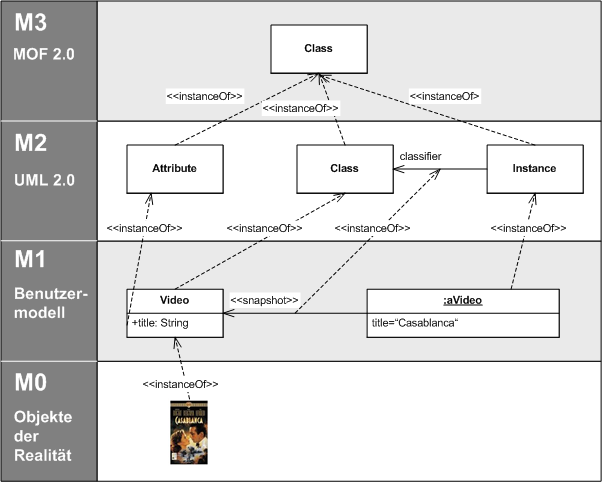
\includegraphics[width=0.75\textwidth]{MOF}
\end{figure}

\newpage
\subsection*{Scientific paper}

\begin{quest}Verklaar de verschillende lagen die we kunnen onderscheiden in het Conceptual Modelling Quality Framework (CMQF).\end{quest}

\begin{enumerate}
    \item Physical layer: bevate de waarneembaare, fysieke elementen van het quality framework.
    \item Knowledge layer: loopt evenwijdig met de physical layer. Echter, waar de physical layer in de `echte wereld' bestaat, bestaat deze knowledge layer enkel cognitief.
    \item Learning layer: meet hoe goed leren, interpretatie en/of het begrijpen plaatsvindt.
    \item Development layer: de elementen van de physical layer hebben hun wortelen op vlak van development in de knowledge layer. De knowledge van een developer wordt gebruikt om de daaropvolgende physical artefacten te maken.
\end{enumerate}

\begin{quest}Gegeven het CMQF, verklaar de volgende termen, positioneer ze in \'e\'en van de lagen van het CMQF en \& illustreer met een eigen voorbeeld.
\end{quest}

\begin{itemize}
    \item Ontological quality (physical layer): de modelling language moet alle modelling concepts kunnen beschrijven.
    \item Syntactic quality (physical layer): alle elementen in het model moeten conform zijn met de taal die gebruikt is.
    \item Semantic quality (physical layer): het model moet kloppen met het modelling domain.
    \item Empirical quality (physical layer): hoe goed is het model leesbaar?
    \item Perceived Semantic quality (knowledge layer): klopt de domain knwoledge met de model interpretation?
    \item View quality (learning layer) hoe goed de stakeholder kennis heeft van het domain knowledge.
    \item Pedagogical quality (learning layer): de stakeholders moeten de juiste `mindset' hebben.
    \item Linguistic quality (learning layer: de stakeholder moet kennis hebben van de modelleertaal.
    \item Pragmatic quality (learning layer): beschrijft het begrijpen van het finale, fysieke model door de stakeholder op vlak van volledigheid en correctheid .
    \item Applied domain knowledge quality (development layer): kennis van het domein is fundamenteel voor alle disciplines. De kwaliteit van de finale representatie is rechtstreeks afhankelijk van de juistheid van communicatie en toepassing van de knowledge.
    \item Applied language knowledge quality (development layer): de kwaliteit van de fysieke representatie van het model is rechtstreeks afhankelijk van de kennis van de modelleertaal.
\end{itemize}

\section{Validation}

NIET TE KENNEN IN ACADEMIEJAAR 2016-2017 (Prof. Geert Poels)\\
(staat in commentaar in het \LaTeX-bestand).
\begin{comment}
\subsection*{Chapter 27: Fundamentals of requirements validation}

\subsubsection{What is the difference between validation and verification?}
\begin{itemize}
	\item Validation: Building the right system: Kijken wat men nodig heeft voor een specifiek project. (With stakeholders, geschiktheid)
	\item Verification: Building the system right: Nakijken of het project wel juist uitgevoerd wordt. (Correct or Incorrect, through proofs)
\end{itemize}

\subsubsection{Validation should occur wwith respect to different dimensions. Which are these and give an example of one or two activities that would belong to a minimal validation (level 1) for that dimension.}
\begin{enumerate}
	\item Content: completeness, correctness
	\item Documentation: Compliance to documentation rules/guidlines
	\item Agreement: checked for conflicts, conflicts resolved
\end{enumerate}

\subsubsection{What are the six important principles of validation and explain each of them briefly.}
\begin{enumerate}
	\item Involving the right stakeholders: internal and external validation concerning the right people.
	\item Separating Defect Detection from Defect Correction: Defect correction depends on the Defect error.
	\item Leveraging multiple independent views
	\item Use of appropriate documentation formats: adapt documentation format to audience
	\item Creation of development artefacts during validation: creation of test scenario's 
	\item Repeated validation 
\end{enumerate}
mnemonic: SLURCI

\subsection*{Chapter 28: Validation techniques}

\subsubsection{What are the essential differences between inspection, desk check and walkthrough in terms of goals, effort and benefit.}

\begin{itemize}
	\item inspection: extensive search for defects in a manageable set of requirements Benefit: High Effort: High-Medium
	\item desk check: less detailed check of a larger set of artefacts, Benefit: Medium, Effort: Medium
	\item walkthrough: feedback on early sketches, elicitation of new ideas, getting agreement. Benefit: Low, Effort, Low-Medium
\end{itemize}

\subsubsection{How can the creation of artefacts contribute to validation ?}
Bij de development van een prototype kunnen goals en scenarios gebruikt worden om te beslissen wat er in het prototype mag komen. Bij het gebruik van het prototype kunnen scenarios gebruikt worden om te valideren of het prototype werkt. Bij de uitvoering kunnen gebruikers hun handelingen of opmerkingen documenteren.

\subsubsection{How can prototyping contribute to validation ? What are the pros and cons of this technique?}
\begin{itemize}
	\item Pro: Early detection of problems, reduce costs, proof of feasibility
	\item Con: Effort can be high, de stakeholder mag niet denken dat omdat er al een prototype is er niet veel werk meer is.
\end{itemize}

\subsubsection{What are the two main kinds of approaches to test case definition and what are their characteristics in terms of applicability to test levels and coverage of the test object?}
\begin{enumerate}
	\item Code-based testing: Applicability: Only component testing. Coverage: Hole code can be covered.
	\item Specification-based testing: Applicability: Alle levels. Coverage: Hole specification can be covered.
\end{enumerate}

\subsubsection{What are the main test-case derivation approaches for requirements-based testing and what are their major characteristics.}
\begin{enumerate}
	\item Direct derivation of Test Cases from requirements artefacts: experience-based selection of test cases
	\item Model-based  Test Case derivation: state machines and flow diagrams.
\end{enumerate}
\end{comment}
\end{document}

